\documentclass[11pt]{article}
% Basic Packages for Encoding (Input AND Output) and Langauge Support
\usepackage[utf8]{inputenc}
\usepackage[T1]{fontenc}
\usepackage[french]{babel}

% Change Layout with a User-Friendly Interface
\usepackage[margin=1in]{geometry}

% Include Pictures with a User-Friendly Interface
\usepackage{graphicx}
\usepackage{float}

% Extended Math Support from the Famous 'American Mathematical Society'
\usepackage{amsmath}
\usepackage{amsfonts}
\usepackage{amssymb}

% Just for Demonstration Purposes
\usepackage[math]{blindtext}

% For use on computer
\usepackage{hyperref}

% For table color
\usepackage{xcolor,colortbl}

% Titre
\usepackage[affil-it]{authblk}
\title{\textbf{TP Addition des résistances}}
\author{Camille Yerly, Fedor Kleymenov, Romain Blondel}
\affil{2M8, Gymnase Auguste Piccard}
\date{28 novembre 2022}

\begin{document}

\maketitle

\section{But}

Le but de cette expérience consiste à vérifier et à comprendre les lois d’addition des résistances en série, en parallèle et mixte dans un circuit électrique.  

\section{Introduction théorique}

Les circuits électriques sont omniprésents dans nos vies. Ils sont dans nos maisons, voitures, appareils électroménagers, et ainsi de suite. Il est donc important de pouvoir prendre des mesures de manière pratique, et de pouvoir prédire ce qui peut l'être. Par exemple, peut-on en connaissant les composants du circuit (comme les résistances, ...), en connaître les mesures pertinentes sans le démonter. Ceci en ne mesurant que la tension totale du circuit, nous pourrions par calcul savoir l'intensité et la tension pour chaque élément de celui-ci. C'est ce que montrent les expériences qui suivent, en comparant des mesures à des calculs théoriques de ce genre.\\

Il subsiste deux structures fondamentales pour le montage des éléments en circuit. Le montage en série et le montage parallèle. Dans notre expérience, il y a un troisième montage qui est mixte. L’ensemble des calculs utilisés proviennent de la loi d’Ohm qui est : $U=R \cdot I$ dont $U$ est la tension aux bornes mesurée en Volt $[V]$, $I$ est l’intensité du courant en Ampère $[A]$ et $R$ est la résistance en Ohm $[\Omega]$. On aura besoin également des lois d’assemblages de résistances en série ou en parallèle, car chaque montage a ses spécificités et ses lois.

\paragraph*{Un circuit en série} est un montage électrique dans lequel les éléments du circuit sont reliés les uns à la suite des autres. Le courant n’a alors qu’un seul chemin possible pour revenir à la source de courant. La propriété principale de ce circuit est la loi d’Unicité qui dit que chaque élément du montage est traversé par le même courant $I$  car tous les dipôles d’un circuit en série sont parcourus par un courant électrique de même intensité. Pour $U$, les tensions aux bornes des éléments s’additionnent pour donner la tension totale. Pour finir la résistance en série, elles s’additionnent pour en former qu’une comme la tension.\\
Donc les formules correspondantes sont :  

$$I_{tot}=I_1=I_2=...=I_n$$
$$U_{tot}= U_1+U_2+...+U_n$$
$$R_{tot}= R_1+R_2+...+R_n$$

\paragraph{Un circuit en parallèle} est un montage électrique dans lequel les appareils sont placés parallèlement les uns aux autres. Le courant peut revenir à la source par plusieurs chemins différents. Chaque élément est traversé par la même tension $U$, les courants s’additionnent pour donner le courant total et pour les résistances en parallèle, elles peuvent être remplacé par une seule résistance équivalente.\\
Les formules correspondantes sont : 

$$U_{tot}=U_1=U_2=...=U_n$$
$$I_{tot}= I_1+I_2+...+I_n$$
$$\frac{1}{R_{equ}}=\frac{1}{R_1}+\frac{1}{R_2}+...+\frac{1}{R_n}$$\\

Pour le circuit mixte, il faut appliquer successivement les lois d’addition en parallèle et en série pour calculer les valeurs des différentes tensions et courants.  

\section{Principe de mesure et description}

Nous avons fait trois expériences distinctes en y relevant les tensions et intensité dans les différentes parties. La première est celle du montage en série, la deuxième en parallèle et la dernière le montage mixte.

\subsection{Matériel}

\begin{itemize}
\item Breadboard (plaque de montage de circuits)
\item Différentes résistances (on utilisera 10, 20, 50, 100 et 200 $[\Omega]$)
\item Deux multimètres
\item Un générateur
\item Des câbles et autres connecteurs (au moins 7 pour le circuit, 2 câbles pour le générateur et 2 par multimètre)
\end{itemize}

\subsection{Déroulement}

Pour chaque cas de montage, il va falloir observer le circuit proposé et dessiner le schéma correspondant, puis mesurer les valeurs de courant et de tension valables pour chaque résistance.Afin de mesurer le courant, l’appareil s’appelle un ampèremètre. Comme le courant électrique représente le flux d’électrons qui circule, l’ampèremètre a besoin que tout le courant le traverse. Il est donc monté en série. Pour la tension, l’appareil qui la mesure s’appelle un voltmètre. Une tension représente une énergie par unité de charge, soit aux bornes d’un appareil, soit aux bornes d’un générateur. Le voltmètre doit ainsi être connecté aux bornes de l’appareil ou du générateur. Il faut par conséquent brancher le voltmètre en parallèle.Dans notre cas, nous avons deux multimètres que nous mettrons sur le mode nécessaire.\\ 
Le montage impacte la façon de mesurer le courant ou la tension, comme vu dans l'introduction.\\

Faisons la démarche de la première expérience, celle des résistances en série :\\

Après avoir observé le circuit proposé, l’avoir dessiné et l’avoir construit sur une plaque (voir figure \ref{fig:pra-1}), nous avons mesuré les valeurs du courant et de la tension valables pour chaque résistance. Par la suite, nous avons calculé dans un ordre donné, la résistance totale, l’intensité du courant et les différentes tensions avec l’aide de la loi d’Ohm et celle de l’assemblage des résistances en série afin de comparer les valeurs obtenues par la mesure et celles calculées. Pour finir, nous avons vérifié la loi d’addition des courants en parallèle.\\  

Cette démarche est valable pour chaque montage, mais nous devons mesurer les valeurs différemment et les calculer dans un autre ordre. Pour la deuxième expérience (voir figure \ref{fig:pra-2}), celle des résistances en parallèle, nous avons dû adapter la façon de mesurer la tension et le courant, puis nous avons dû calculer les valeurs dans cet ordre : la résistance totale, la tension totale et les différentes intensités du courant.\\
Pour la troisième expérience (voir figure \ref{fig:pra-3}), celle du montage des résistances mixtes, nous avons dû également adapter la façon de mesurer la tension et le courant, puis nous avons dû calculer les valeurs dans cet ordre : la résistance totale en deux étapes, d’abord en série puis en parallèle, la tension totale et la tension pour chaque groupe, et pour finir les différentes intensités du courant.\\  

\subsection{Schémas}

Dans les schémas qui suivent,  les diverses connexions sont représentées sur les breadboards. Tout d'abord, le générateur au circuit (G, avec les câbles bleu et rouges), puis les résistances avec leurs valeurs respectives (en gris) et les connecteurs en blanc et noir (ceux en noir vont servir à mettre l’ampèremètre à leur place afin de mesurer l'intensité du courant, et le voltmètre se branche aux carrés de chaque côté de la résistance).

\begin{figure}[H]
\centering
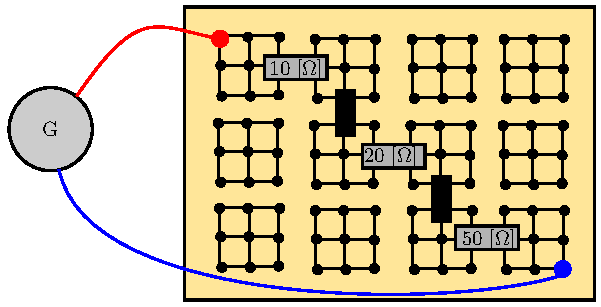
\includegraphics[scale=1]{images/schm-pra/schm1.pdf}
\caption{Schéma pratique du $1^{er}$ montage}
\label{fig:pra-1}
\end{figure}

\begin{figure}[H]
\centering
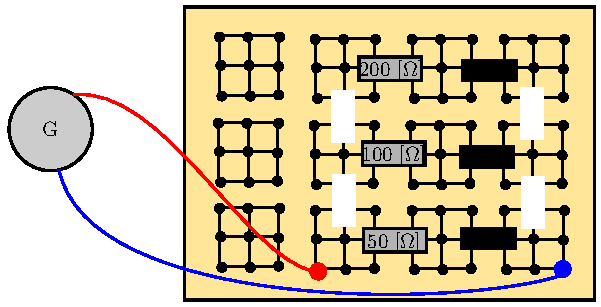
\includegraphics[scale=1]{images/schm-pra/schm2.pdf}
\caption{Schéma pratique du $2^{e}$ montage}
\label{fig:pra-2}
\end{figure}

\begin{figure}[H]
\centering
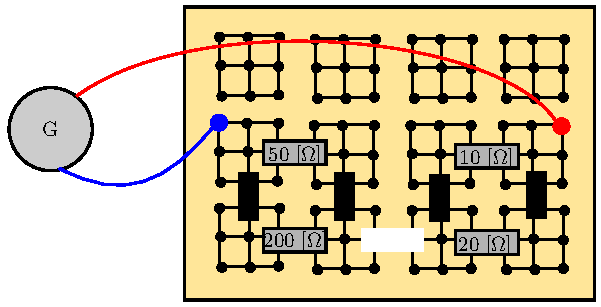
\includegraphics[scale=1]{images/schm-pra/schm3.pdf}
\caption{Schéma pratique du $3^{e}$ montage}
\label{fig:pra-3}
\end{figure}

\section{Résultats et calculs}

Les résistances totales des différents circuits n'ont pas été mesurées. Les indices dans les calculs sont les mêmes que pour la mesure, donc les tensions et intensité $U_n$ et $I_n$ sont celles aux bornes, respectivement dans la boucle, de la résistance $R_n$. Pour le montage mixte, on a mesuré les tensions et intensités aux bornes des groupes de résistances indiquées, mais la résistance de ces groupes n'a pas été mesurée.\\
Chaque montage est accompagné d'un schéma théorique de celui-ci pour permettre une meilleure compréhension des calculs.Ceux-ci seront effectué en utilisant les valeurs de résistances et de tensions totale pour en déduire le reste.

\subsection{Montage 1 : Résistance en série}

\begin{figure}[H]
\centering
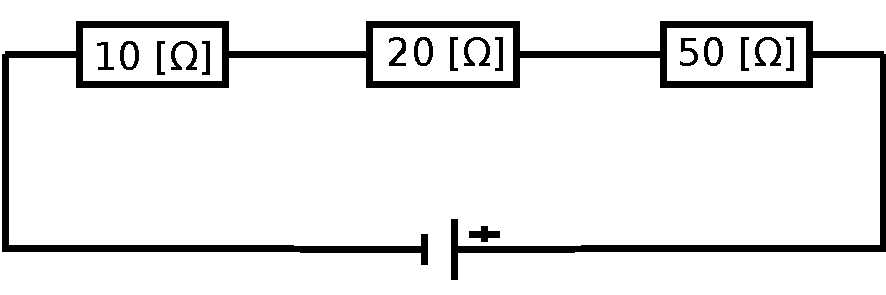
\includegraphics[scale=0.5]{images/elec-schem/montage1_1.pdf}
\caption{Schéma théorique du premier montage}
\label{fig:th-1}
\end{figure}

\subsubsection*{Mesures}

\begin{table}[H]
\center
\begin{tabular}{|>{\columncolor{gray}}c||c|>{\columncolor{lightgray}}c|c||>{\columncolor{lightgray}}c|}
\hline
\rowcolor{gray} \cellcolor{black} & 1 & 2 & 3 & Total\\ \hline
$R \ [\Omega]$ & 10 & 20 & 50 & x \\ \hline
$U \ [V]$ & 1.259 & 2.512 & 6.23 & 10 \\ \hline
$I \ [A]$ & 0.126 & 0.126 & 0.126 & 0.126 \\ \hline
\end{tabular}
\caption{Mesures dans le premier montage}
\label{table:mesures_m1}
\end{table}

\subsubsection*{Calculs}

Le montage étant en série, on sait que la sommes des résistances correspond à celle totale du système $R_{tot} = R_1 + R_2 + R_3$. De là, via la loi d'Ohm $U=R \cdot I \Leftrightarrow I = \frac{U}{R}$, on calcule $I_{tot} = \frac{U_{tot}}{R_{tot}}$, puis on calcule chaque tension aux bornes des résistance $U_n = R_n \cdot I_n = R_n \cdot I_{tot}$, car comme dit dans l'introduction $I_{tot} = I_1 = I_2 = I_3$.

\begin{table}[H]
\center
\begin{tabular}{|>{\columncolor{gray}}c||c|>{\columncolor{lightgray}}c|c||>{\columncolor{lightgray}}c|}
\hline
\rowcolor{gray} \cellcolor{black} & 1 & 2 & 3 & Total\\ \hline
$R \ [\Omega]$ & 10 & 20 & 50 & 80 \\ \hline
$U \ [V]$ & 1.25 & 2.5 & 6.25 & 10 \\ \hline
$I \ [A]$ & 0.125 & 0.125 & 0.125 & 0.125 \\ \hline
\end{tabular}
\caption{Calculs dans le premier montage}
\label{table:calculs_m1}
\end{table}

\subsection{Montage 2 : Résistance en parallèle}

\begin{figure}[H]
\centering
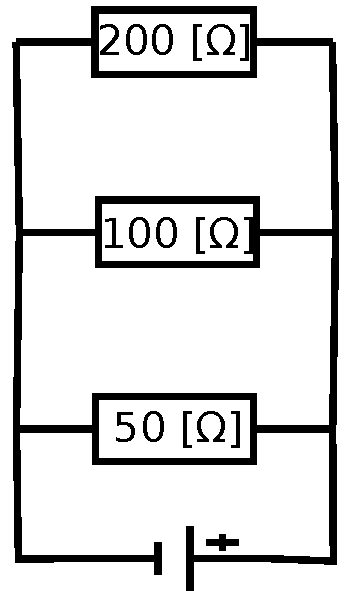
\includegraphics[scale=0.5]{images/elec-schem/montage2_1.pdf}
\caption{Schéma théorique du second montage}
\label{fig:th-2}
\end{figure}

\subsubsection*{Mesures}

\begin{table}[H]
\center
\begin{tabular}{|>{\columncolor{gray}}c||c|>{\columncolor{lightgray}}c|c||>{\columncolor{lightgray}}c|}
\hline
\rowcolor{gray} \cellcolor{black} & 1 & 2 & 3 & Total\\ \hline
$R \ [\Omega]$ & 50 & 100 & 200 & x \\ \hline
$U \ [V]$ & 8.47 & 8.48 & 8.48 & 8.47 \\ \hline
$I \ [A]$ & 0.172 & 0.086 & 0.043 & 0.3 \\ \hline
\end{tabular}
\caption{Mesures dans le second montage}
\label{table:mesures_m2}
\end{table}

\subsubsection*{Calculs}

Le montage étant en parallèle, on peut utiliser la formule $\frac{1}{R_{tot}}=\frac{1}{R_1}+\frac{1}{R_2}+\frac{1}{R_3} \Leftrightarrow R_{tot}=\frac{1}{\frac{1}{R_1}+\frac{1}{R_2}+\frac{1}{R_3}}$ pour calculer la résistance totale. Ensuite, via $U=R \cdot I \Leftrightarrow I = \frac{U}{R}$, on obtient l'intensité totale, ainsi que les différentes intensités au niveau de chaque boucle. 

\begin{table}[H]
\center
\begin{tabular}{|>{\columncolor{gray}}c||c|>{\columncolor{lightgray}}c|c||>{\columncolor{lightgray}}c|}
\hline
\rowcolor{gray} \cellcolor{black} & 1 & 2 & 3 & Total\\ \hline
$R \ [\Omega]$ & 50 & 100 & 200 & 28.571 \\ \hline
$U \ [V]$ & 8.47 & 8.47 & 8.47 & 8.47 \\ \hline
$I \ [A]$ & 0.169 & 0.085 & 0.042 & 0.296 \\ \hline
\end{tabular}
\caption{Calculs dans le second montage}
\label{table:calculs_m2}
\end{table}

\subsection{Montage 3 : Mixte}

\begin{figure}[H]
\centering
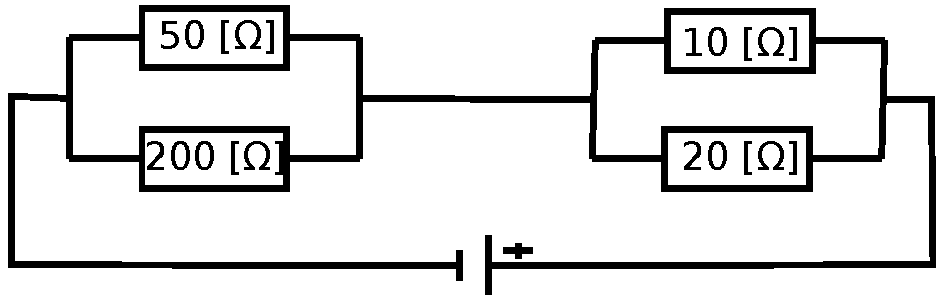
\includegraphics[scale=0.5]{images/elec-schem/montage3_1.pdf}
\caption{Schéma théorique du troisième montage}
\label{fig:th-3}
\end{figure}

\subsubsection*{Mesures}

\begin{table}[H]
\center
\begin{tabular}{|>{\columncolor{gray}}c||c|>{\columncolor{lightgray}}c|c|>{\columncolor{lightgray}}c||c|>{\columncolor{lightgray}}c||c|}
\hline
\rowcolor{gray} \cellcolor{black} & 1 & 2 & 3 & 4 & A (1 et 2) & B (3 et 4) & Total\\ \hline
$R \ [\Omega]$ & 50 & 200 & 10 & 20 & x & x & x \\ \hline
$U \ [V]$ & 8.56 & 8.56 & 1.449 & 1.449 & 8.56 & 1.449 & 10 \\ \hline
$I \ [A]$ & 0.174 & 0.043 & 0.145 & 0.073 & 0.217 & 0.217 & 0.217 \\ \hline
\end{tabular}
\caption{Mesures dans le troisième montage}
\label{table:mesures_m3}
\end{table}

\subsubsection*{Calculs}

Pour les mesures et les calculs, il est utile de prendre les deux boucles en parallèles comme une unique résistance, avec donc $\frac{1}{R_A} = \frac{1}{R_1} + \frac{1}{R_2} \Leftrightarrow R_A = \frac{1}{\frac{1}{R_1} + \frac{1}{R_2}}$ et $\frac{1}{R_B} = \frac{1}{R_3} + \frac{1}{R_4} \Leftrightarrow R_B = \frac{1}{\frac{1}{R_3} + \frac{1}{R_4}}$. De là, vu que ces groupes sont en séries, on obtient $R_{tot} = R_A + R_B$, puis on réutilise $I_{tot} = \frac{U_{tot}}{R_{tot}}$ pour calculer l'intensité. Ensuite, la tension des différents groupes se déduit de la loi d'Ohm $U=R \cdot I$, car $I_{tot} = I_A = I_B$, par $U_A = R_A \cdot I_{tot}$ (et $U_B = R_B \cdot I_{tot}$). En connaissant la tension de chaque groupe, qui est la même au sein de celui-ci, on peut calculer les intensités dans chaque boucle (par exemple $I_1 = \frac{U_A}{R_1}$).

\begin{table}[H]
\center
\begin{tabular}{|>{\columncolor{gray}}c||c|>{\columncolor{lightgray}}c|c|>{\columncolor{lightgray}}c||c|>{\columncolor{lightgray}}c||c|}
\hline
\rowcolor{gray} \cellcolor{black} & 1 & 2 & 3 & 4 & A (1 et 2) & B (3 et 4) & Total\\ \hline
$R \ [\Omega]$ & 50 & 200 & 10 & 20 & 40 & 6.667 & 46.667 \\ \hline
$U \ [V]$ & 8.571 & 8.571 & 1.429 & 1.429 & 8.571 & 1.429 & 10 \\ \hline
$I \ [A]$ & 0.171 & 0.043 & 0.143 & 0.071 & 0.214 & 0.214 & 0.214 \\ \hline
\end{tabular}
\caption{Calculs dans le troisième montage}
\label{table:calculs_m3}
\end{table}

\subsection{Erreur}

Nous voyons déjà dans les tableau d'assez faibles écarts entre les mesures et le calcul théorique. Il demeure intéressant de le quantifier, en comparant les tensions et intensité pour chaque circuit. Cela n'est pas nécessaire pour les résistances, car elles n'ont pas été mesurées par nous et été prises en tant que valeur fixe dans les calculs. Il en va de même pour la tension totale du circuit qui est la seule mesure dont on se sert pour poser les calculs.

\begin{table}[H]
\center
\begin{tabular}{|>{\columncolor{gray}}c||c|>{\columncolor{lightgray}}c|c||>{\columncolor{lightgray}}c|}
\hline
\rowcolor{gray} \cellcolor{black} & 1 & 2 & 3 & Total\\ \hline
$\Delta U \ [\%]$ & 0.72 & 0.48 & 0.32 & x \\ \hline
$\Delta I \ [\%]$ & 0.80 & 0.80 & 0.80 & 0.80 \\ \hline
\end{tabular}
\caption{Erreur dans le premier montage}
\label{table:erreur_m1}
\end{table}

\begin{table}[H]
\center
\begin{tabular}{|>{\columncolor{gray}}c||c|>{\columncolor{lightgray}}c|c||>{\columncolor{lightgray}}c|}
\hline
\rowcolor{gray} \cellcolor{black} & 1 & 2 & 3 & Total\\ \hline
$\Delta U \ [\%]$ & 0.00 & 0.12 & 0.12 & x \\ \hline
$\Delta I \ [\%]$ & 1.53 & 1.53 & 1.53 & 1.20 \\ \hline
\end{tabular}
\caption{Erreur dans le second montage}
\label{table:erreur_m2}
\end{table}

\begin{table}[H]
\center
\begin{tabular}{|>{\columncolor{gray}}c||c|>{\columncolor{lightgray}}c|c|>{\columncolor{lightgray}}c||c|>{\columncolor{lightgray}}c||c|}
\hline
\rowcolor{gray} \cellcolor{black} & 1 & 2 & 3 & 4 & A (1 et 2) & B (3 et 4) & Total\\ \hline
$\Delta U \ [\%]$ & 0.13 & 0.13 & 1.43 & 1.43 & 0.13 & 1.43 & x \\ \hline
$\Delta I \ [\%]$ & 1.50 & 0.33 & 1.50 & 2.20 & 1.27 & 1.27 & 1.27 \\ \hline
\end{tabular}
\caption{Erreur dans le troisième montage}
\label{table:erreur_m3}
\end{table}

Nous voyons donc des mesures qui sont globalement d'excellente précision, avec une erreur inférieure à $2 \ [\%]$ pour toutes à l'exception d'une (à $2.20 \ [\%]$) et presque une moitié des mesures précises à $1 \ [\%]$ près.

\subsection{Incertitudes} \label{subsec:incert}

Les résistances sont spécifiées à une précision de $1 [\% ]$. Nous évaluons également l'incertitude du générateur autour des $2 [\% ]$ en comparant la valeur donnée par le multimètre à celle affichée par le générateur. Les câbles et les connecteurs étant aussi une cause d'incertitude, leur multiplication dans la deuxième et la troisième expérience justifient donc une augmentation de l'erreur par rapport aux valeurs attendues. 

\section{Discussion des résultats}

Les prédictions correspondent assez bien aux valeurs mesurées. En effet, l'erreur sur nos résultats varie entre $0.12 \ [\% ]$ et $2.20 \ [\% ]$. Nous remarquons une légère augmentation de celle-ci dans les dernières expériences causée par la complexification des circuits (voir Section \ref{subsec:incert}). Malgré cela, la différence par rapport aux valeurs théoriques restent à l'intérieur des incertitudes liés aux divers composants et au montage. Les valeurs mesurées correspondant aux valeurs théoriques sont une validation de la loi $U=R \cdot I$, cette loi étant fondamentale pour le bon fonctionnement de tout circuit électronique, ainsi que les lois d'additions des résistances qui en découlent.\\
On remarque également que la déduction des tensions est globalement plus précise que celle des intensités (voir tables \ref{table:erreur_m1}, \ref{table:erreur_m2} et \ref{table:erreur_m3}). Il faut aussi noter qu'avec les instruments que nous avions à disposition, sur le même montage, il semble que plus la résistance est élevée, plus la prédiction est précise (voir la table \ref{table:erreur_m3} et comparer les tables \ref{table:mesures_m3} et \ref{table:calculs_m3}). Il est même intéressant de remarquer que sans garder les décimales supplémentaires, la prédiction de l'intensité sur la résistance de $200 \ [\Omega]$, est exacte en ne considérant que les chiffres dits significatifs.\\\\
Il demeure néanmoins des sources d'erreurs pouvant expliquer les différences observées. Tout d'abord, les résistances n'ont pas été contrôlées avant mesures. Ensuite, l'intensité et la tension totale délivrée par le générateur auraient pu être mesurées et calibrées de manière plus précise. En effet, ce dernier n'indiquait pas exactement les même valeurs que le multimètre. De plus, on voit que le modèle n'est pas parfait et on ne prend, par exemple, pas en compte les résistances des différents composants tel que les connecteurs (cela se voit dans la mesure de tension censée être constante dans la table \ref{table:mesures_m2}). Finalement, on considère que la mise des instruments de mesure ne perturbe pas le circuit du tout, ce qui n'est pas complètement réaliste, mais négligeable. Il faut quand même noter qu'une mesure de l'intensité en milliampère aurait peut-être pu être plus pertinente afin d'être plus précis et de permettre une comparaison plus fine.

\section{Conclusion}

Cette expérience s'avère concluante : tous les objectifs ont été atteint. Nous avons pu vérifier la loi d'Ohm ainsi que les lois d’addition des résistances en série, en parallèle et mixte dans un circuit électrique. et bien que l'expérience ait offert d'excellents résultats il serait possible de l'optimiser en améliorant le matériel électronique en faisant, par exemple, réaliser une maintenance et une re-calibration du générateur et du multimètre, principales sources d'incertitudes, par un laboratoire accrédité. De plus, il serait intéressant de faire une mesure des résistances, ainsi que des mesures plus fines, afin de confirmer d'autant plus les résultats obtenus et de voir jusqu'à quel point on peut utiliser cette théorie avec les approximations faites, tel que l'absence de résistance des câbles. Néanmoins, nous voyons que, via la mesure de la tension et en connaissant les composants d'un circuit, il est possible d'en prédire de manière assez précise les autres données pertinentes.

\end{document}